\documentclass[]{article}
\usepackage{lmodern}
\usepackage{amssymb,amsmath}
\usepackage{ifxetex,ifluatex}
\usepackage{fixltx2e} % provides \textsubscript
\ifnum 0\ifxetex 1\fi\ifluatex 1\fi=0 % if pdftex
  \usepackage[T1]{fontenc}
  \usepackage[utf8]{inputenc}
\else % if luatex or xelatex
  \ifxetex
    \usepackage{mathspec}
  \else
    \usepackage{fontspec}
  \fi
  \defaultfontfeatures{Ligatures=TeX,Scale=MatchLowercase}
\fi
% use upquote if available, for straight quotes in verbatim environments
\IfFileExists{upquote.sty}{\usepackage{upquote}}{}
% use microtype if available
\IfFileExists{microtype.sty}{%
\usepackage[]{microtype}
\UseMicrotypeSet[protrusion]{basicmath} % disable protrusion for tt fonts
}{}
\PassOptionsToPackage{hyphens}{url} % url is loaded by hyperref
\usepackage[unicode=true]{hyperref}
\PassOptionsToPackage{usenames,dvipsnames}{color} % color is loaded by hyperref
\hypersetup{
            pdftitle={CSDE 502 Winter 2021, Assignment 10},
            pdfauthor={dcoomes},
            colorlinks=true,
            linkcolor=Maroon,
            citecolor=Blue,
            urlcolor=blue,
            breaklinks=true}
\urlstyle{same}  % don't use monospace font for urls
\usepackage[margin=1in]{geometry}
\usepackage{graphicx,grffile}
\makeatletter
\def\maxwidth{\ifdim\Gin@nat@width>\linewidth\linewidth\else\Gin@nat@width\fi}
\def\maxheight{\ifdim\Gin@nat@height>\textheight\textheight\else\Gin@nat@height\fi}
\makeatother
% Scale images if necessary, so that they will not overflow the page
% margins by default, and it is still possible to overwrite the defaults
% using explicit options in \includegraphics[width, height, ...]{}
\setkeys{Gin}{width=\maxwidth,height=\maxheight,keepaspectratio}
\IfFileExists{parskip.sty}{%
\usepackage{parskip}
}{% else
\setlength{\parindent}{0pt}
\setlength{\parskip}{6pt plus 2pt minus 1pt}
}
\setlength{\emergencystretch}{3em}  % prevent overfull lines
\providecommand{\tightlist}{%
  \setlength{\itemsep}{0pt}\setlength{\parskip}{0pt}}
\setcounter{secnumdepth}{5}
% Redefines (sub)paragraphs to behave more like sections
\ifx\paragraph\undefined\else
\let\oldparagraph\paragraph
\renewcommand{\paragraph}[1]{\oldparagraph{#1}\mbox{}}
\fi
\ifx\subparagraph\undefined\else
\let\oldsubparagraph\subparagraph
\renewcommand{\subparagraph}[1]{\oldsubparagraph{#1}\mbox{}}
\fi

% set default figure placement to htbp
\makeatletter
\def\fps@figure{htbp}
\makeatother

\usepackage{booktabs}
\usepackage{longtable}
\usepackage{array}
\usepackage{multirow}
\usepackage{wrapfig}
\usepackage{float}
\usepackage{colortbl}
\usepackage{pdflscape}
\usepackage{tabu}
\usepackage{threeparttable}
\usepackage{threeparttablex}
\usepackage[normalem]{ulem}
\usepackage{makecell}
\usepackage{xcolor}

\title{CSDE 502 Winter 2021, Assignment 10}
\author{\href{mailto:dcoomes@uw.edu}{dcoomes}}
\date{}

\begin{document}
\maketitle

{
\hypersetup{linkcolor=black}
\setcounter{tocdepth}{2}
\tableofcontents
}
\section{Introduction}\label{introduction}

Despite considerable progress since 1990, approximately 5.2 million
children under the age of five died worldwide in 2019.(UNICEF 2020) The
most dangerous time for children under five is the neonatal period (the
first month of life) . The chance of death after the first month and
before the first year is slightly higher than the chance of death
between 1-5 years of age.(UNICEF 2020)

Spain has one of the lowest under five (u5) mortality rates in Europe.
The u5 mortality rate in Spain (2.7 deaths per 1,000 live births) is
lower than that of the European Union average (3.5 per 1,000 live
births) and much lower than that of the United States (5.7 per 1,000
live births).(INED 2021) Like many other countries, child mortality in
Spain has reduced considerably since the beginning of the 20th century.
In this analysis, we will examine mortality among children under five
years of age in Spain over the last 108 years, and examine trends among
male and female children during this time.

\section{Methods}\label{methods}

\subsection{Data}\label{data}

The data used in this analysis is from the \emph{Human Mortality
Database} curated by the Max Planck Institute for Demographic Research.
This database was designed to provide mortality data for various
investigators, including researchers and students. For this analysis we
use the mortality dataset from Spain from 1908 - 2018. The dataset we
use reports aggregated deaths over five year periods for each five year
age group. We limit our analysis to those aged 0-1 years and those aged
1-5 years. This dataset and others are available on the
\href{https://www.mortality.org}{Human Mortality Database website}

\subsection{Analysis}\label{analysis}

In this analysis we show the total number of deaths among children under
five years of age in Spain from 1910 - 2018. We show the total number of
deaths for children under 1 year of age and children aged 1-4
separately. We also show the total number of deaths among male and
female children separately.

\section{Results}\label{results}

As is evident in \textbf{Figure 1} the total number of deaths among
children under 1 year and children 1-4 years of age has steadily
decreased from 1910 to 2018. During this entire time span the total
deaths among children under 1 year has been higher than the total deaths
among children aged 1-4. The total deaths decreased dramatically between
1920 and 1965 and have been decreasing more slowly since 1965.

\begin{figure}
\centering
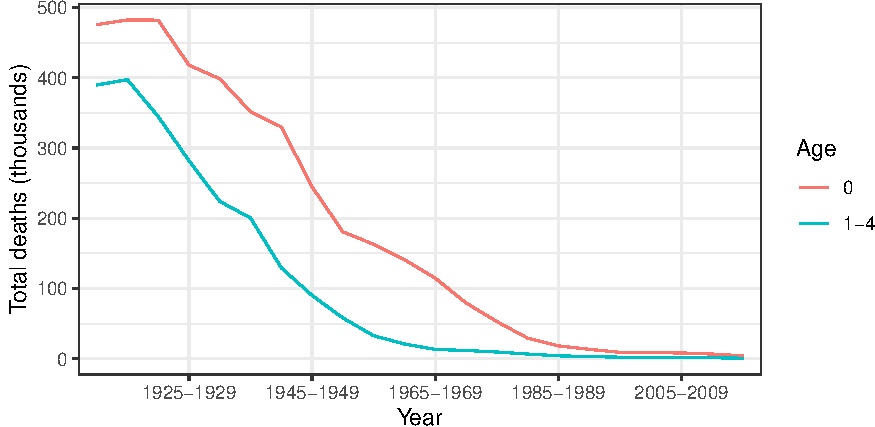
\includegraphics{dcoomes_hw_10_files/figure-latex/ageall-1.pdf}
\caption{Total deaths for age 0 and age 1-4 in Spain from 1910-2018}
\end{figure}

\textbf{Figure 2} shows the difference in total deaths for males and
females, also disagregated by age. For both age groups there were more
male child deaths as compared to female child deaths. The gap between
absolute male deaths and female deaths has decreased as the total number
of deaths has decreased, however, \textbf{Table 1} shows that the
relative gap has remained similar over time.

\begin{figure}
\centering
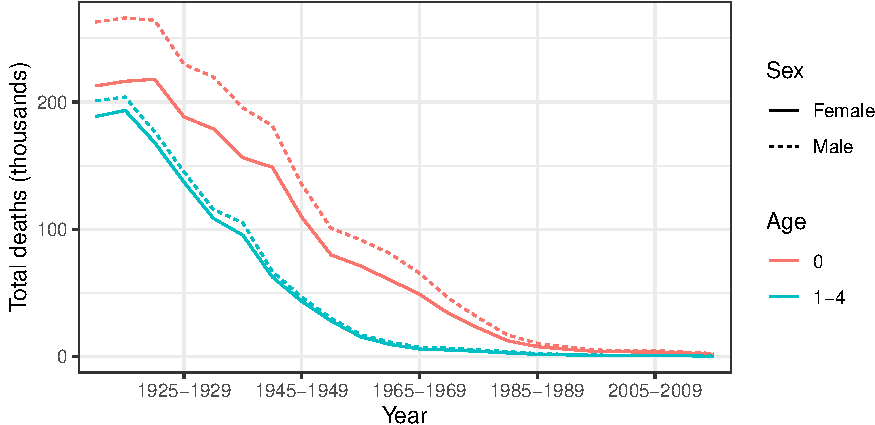
\includegraphics{dcoomes_hw_10_files/figure-latex/sexmort-1.pdf}
\caption{Total deaths for males and females age 0 and age 1-4 in Spain
from 1910-2018}
\end{figure}

The relative proportion of child deaths under age one has remained
relatively stable from 1908 - 2018. Female deaths have ranged from
42.5\% to 45.6\% of overall during this time. There does seem to be a
small trend in female deaths relative to male decreasing between 1920 to
1980 and then increasing again slightly. The overall proportion of
female deaths among children aged 1-4 was similar to those under one
year of age.

\begin{table}

\caption{\label{tab:deathtable}Deaths for infants age 0 in Spain by 5-year age span for males and females}
\begin{tabular}[t]{l|r|r|r|r}
\hline
Year & Female & Male & Female \% & Male \%\\
\hline
1908-1909 & 91,878 & 113,725 & 44.7 & 55.3\\
\hline
1910-1914 & 212,698 & 262,909 & 44.7 & 55.3\\
\hline
1915-1919 & 216,320 & 266,105 & 44.8 & 55.2\\
\hline
1920-1924 & 217,885 & 264,197 & 45.2 & 54.8\\
\hline
1925-1929 & 188,319 & 229,734 & 45.0 & 55.0\\
\hline
1930-1934 & 178,918 & 219,670 & 44.9 & 55.1\\
\hline
1935-1939 & 156,287 & 195,541 & 44.4 & 55.6\\
\hline
1940-1944 & 148,811 & 181,309 & 45.1 & 54.9\\
\hline
1945-1949 & 109,605 & 135,223 & 44.8 & 55.2\\
\hline
1950-1954 & 79,889 & 100,846 & 44.2 & 55.8\\
\hline
1955-1959 & 71,193 & 91,823 & 43.7 & 56.3\\
\hline
1960-1964 & 60,234 & 80,920 & 42.7 & 57.3\\
\hline
1965-1969 & 49,082 & 65,688 & 42.8 & 57.2\\
\hline
1970-1974 & 33,828 & 45,759 & 42.5 & 57.5\\
\hline
1975-1979 & 22,503 & 30,506 & 42.5 & 57.5\\
\hline
1980-1984 & 12,467 & 16,949 & 42.4 & 57.6\\
\hline
1985-1989 & 7,817 & 10,533 & 42.6 & 57.4\\
\hline
1990-1994 & 5,818 & 7,654 & 43.2 & 56.8\\
\hline
1995-1999 & 4,043 & 5,206 & 43.7 & 56.3\\
\hline
2000-2004 & 3,765 & 4,801 & 44.0 & 56.0\\
\hline
2005-2009 & 3,657 & 4,734 & 43.6 & 56.4\\
\hline
2010-2014 & 3,074 & 3,674 & 45.6 & 54.4\\
\hline
2015-2018 & 1,871 & 2,405 & 43.8 & 56.2\\
\hline
\end{tabular}
\end{table}

\textbf{Figure 3A} shows more recent trends in child deaths that cannot
be seen when looking at overall deaths from 1910 - 2018. It shows that
the reduction in deaths continues for both age groups over the time
period of 1985 - 2014. \textbf{Figure 4B} shows a similar trend among
males and females.

\begin{figure}
\centering
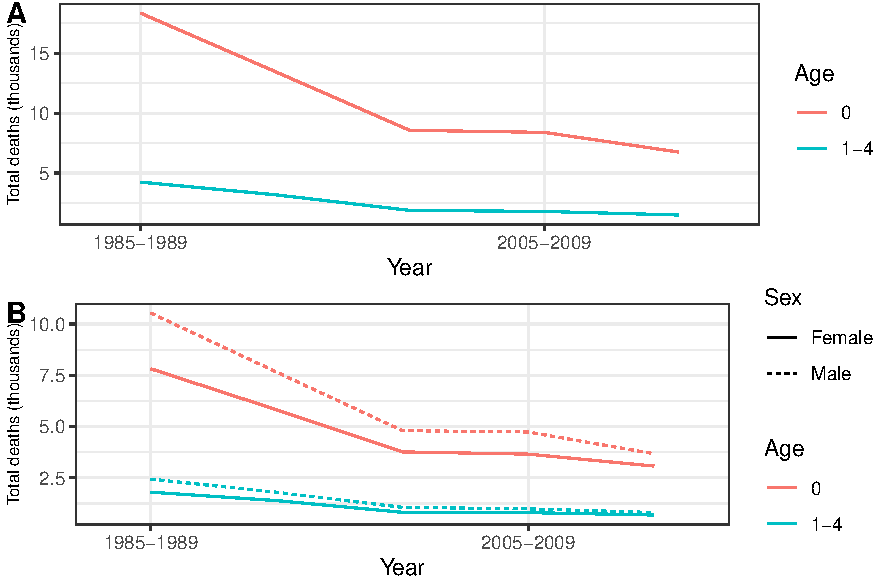
\includegraphics{dcoomes_hw_10_files/figure-latex/recent-1.pdf}
\caption{Total deaths for age 0 and age 1-4 in Spain from 1985-2018}
\end{figure}

\section{Discussion}\label{discussion}

The number of deaths among Spanish children aged below five has steadily
decreased over the past 100 years. In this study we use the absolute
number of deaths, which does not necessarily show a decrease in the
mortality rate. For example, if the birth rate decreased during this
time, then we would see a decrease in the number of deaths even if the
mortality rate remained constant. Previous studies have shown a
reduction in child mortality in Spain over the last 100 years, but also
a reduction in the birth rate from 1970 - 2000. Since 2000, the birth
rate has remained relatively stable, lending evidence that the reduction
in deaths is caused by a reduction in child mortality rates.

The proportion of deaths among male and female infants has remained
relatively stable over the last 100 years in Spain, with male babies
accounting for about 55\% of all under five deaths. This proportion is
similar among those under one year of age and those aged 1-4 years.
Previous research has shown that male babies have a biological
disadvantage in survival as compared to female babies, however, this
disadvantage does not necessarily lead to reduced survival for male
babies as there may be other factors, such as cultural preferences for
males, that lead to differential distribution of resources for children
under five based on sex.(Byass 2012) In the Spanish population over the
last 100 years, based on our analysis, male children under five do have
a survival disadvantage compared to female children.

\section{Conclusion}\label{conclusion}

The number of deaths among children under the age of five in Spain has
decreased over the last 100 years, however, the proportion of male and
female deaths has remained relatively stable.

\newpage

\section*{References}\label{references}
\addcontentsline{toc}{section}{References}

\hypertarget{refs}{}
\hypertarget{ref-Byass2012}{}
Byass, Peter. 2012. ``Child Mortality Estimation: Estimating Sex
Differences in Childhood Mortality since the 1970s.'' \emph{PLoS
Medicine} 9 (8).

\hypertarget{ref-INED}{}
INED, The French Institute for Demographic Studies. 2021. ``Births,
deaths and infant mortality.''
\url{https://www.ined.fr/en/everything_about_population/data/europe-developed-countries/birth-death-infant-mortality/}.

\hypertarget{ref-UNICEF2020}{}
UNICEF. 2020. ``Under-five mortality.''
\url{https://data.unicef.org/topic/child-survival/under-five-mortality/\#status}.

\end{document}
